\chapter{Complex Numbers}

\section{History -
(\href{https://www.youtube.com/watch?v=cUzklzVXJwo}{Veritasium's video},
\href{https://youtu.be/UeRNIxt8o00}{KRN's video})}
Most students encounter complex numbers for the first time when trying to solve quadratic equations.
The roots of the quadratic eqeation $ax^2+bx+c = 0$ are given by the famous formula $\frac{-b \pm \sqrt{b^2-4ac}}{2a}$. When $b^2-4ac < 0$, we need to take the square root of negative numbers in order to compute the roots.  
There is a popular misconception that complex numbers were invented in order to obtain roots to such quadratic equations.
This is inaccurate and it was the roots to cubic equations that prompted the introduction of complex numbers.

The early history of complex numbers is fascinating and it contains all the elements of a good story including competition, intrigue, and deceit. I would highly suggest that you begin
by understanding their history before learning about how to do arithmetic with complex numbers.
In addition to the fact that it is an interesting story, there is a lesson to learn from this history about how we use complex numbers today.
Either of the two videos linked above is a good starting point.

We will use the letter $j$ to refer to the imaginary number $\sqrt{-1}$.
Even though $j$ is not a real number, we can perform all arithmetic operations such as addition, subtraction, multiplication, division with $j$ using the algebra of real numbers keeping in mind that $j^2=-1$.

\section{Cartesian Form - (\href{https://youtu.be/fUEwjQBs6FU}{Video},
\href{https://colab.research.google.com/drive/1IPisKbolmXp2UD7ZuxIRhMEjvaq_Q82G?usp=sharing}{Python notebook})}

A complex number $z$ is any number of the form $z = x+jy$, where $x$ is called the real part of $z$ and $y$ is called the imaginary part of $z$.
The real and imaginary parts are denoted by $\Re\{z\}$ and $\Im\{z\}$, respectively.
Note: The imaginary part is not $jy$, rather it is only $y$.
It is important to stick to this terminology, otherwise computations can go wrong.
Just like how real numbers can be represented on the number line, a complex number
can be represented as a point in a 2-D plane called the complex plane.
The complex plane, shown in Fig.~\ref{fig:argand}, is called the Argand diagram (named after a mathematician).
The complex number $z$ can be thought of as a point with the $X$-coordinate given by the real part of $z$ and the $Y$-coordinate given by the imaginary part of $z$.
Often, it is useful to think of a complex number $z = x+jy$ as a two-dimensional vector where $x$ is the $X$-coordinate and $y$ is $Y$-coordinate of the vector.
%Due to this relationship between a complex number and the corresponding vector, we will abuse the terminology and use the terms complex number and vector interchangeably, if the context should resolve any possible ambiguity.
%the real part of $z$ represents the $X$-coordinate and the imaginary part of $z$
%represents the $Y$-coordinate.
%For example, a complex number is said to lie in the first quadrant (or, second quadrant etc) if the corresponding vector lies in the first quadrant (or, second quadrant etc).

\begin{figure}[h]
\begin{center}
%\includegraphics[width=3.0in]{../Images/ComplexNumbers/complexnumbercartesian}
%\documentclass[%
%% border=1pt
%  border={0pt 0pt 0pt 0pt} % left bottom right top
%]{standalone}
%\usepackage{tikz} % Required for drawing custom shapes
%\usepackage{pgfplots}
%\pgfplotsset{compat = newest}
%
%\usepackage{amsbsy}
%\usetikzlibrary{decorations.pathreplacing,calc}
%\usetikzlibrary{shapes}
%\usepackage{amsmath,stackrel}
%\usetikzlibrary{arrows.meta}
%\usetikzlibrary{arrows}
%\usetikzlibrary{calc}
%\usetikzlibrary{math}
%
%\begin{document}
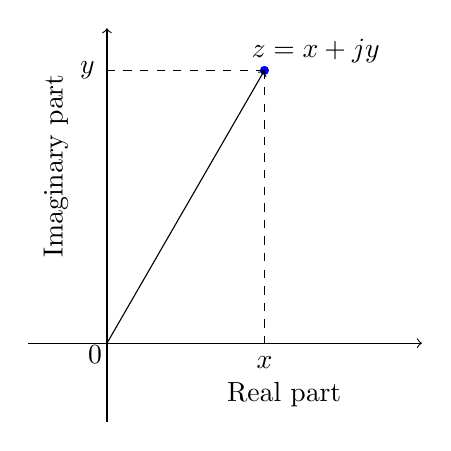
\begin{tikzpicture}
\draw[black,->] (-1,0) -- (4,0);
\draw[black,->] (0,-1) -- (0,4);
\draw[fill,blue] (2,{2*sqrt(3)}) circle[radius=0.05];
\node[align=left,rotate=90] at (-0.65,2.25){Imaginary part};
\node[align=left,rotate=0] at (2.25,-0.65){Real part};
\node at (-0.15,-0.15){0};
\draw[black,->] (0,0) -- (2,{2*sqrt(3)});
\node at (2.65,{2*sqrt(3)+0.25}) {$z = x + j y$};
\draw[dashed] (2,{2*sqrt(3)}) -- (0,{2*sqrt(3)});
\draw[dashed] (2,{2*sqrt(3)}) -- (2,0);
\node at (2,-0.25){$x$};
\node at (-0.25,{2*sqrt(3)}){$y$};
\end{tikzpicture}
%\end{document}
\caption{Argand diagram showing a complex number as a point/vector in the 2-D complex plane}
\label{fig:argand}
\end{center}
\end{figure}

\section{Magnitude and Phase (\href{https://youtu.be/LHkYGsBxue4}{Video})}
The $X$ and $Y$ coordinates of $z$ can be expressed in terms of the length of the vector $r$ and the angle made by this vector with the positive $X$-axis, namely $\theta$. Since $x = r \cos \theta$ and $y = r \sin \theta$, $z$ can be expressed as
\begin{equation}
\label{eqn:polar1}
z = r \cos\theta + j r \sin\theta,
\end{equation}
where $\theta$ can be in degrees or radians (usually radians) and recall that $2 \pi \mbox{ rad } = 360\,^\circ$. $r$ is called the magnitude of $z$, denoted by $|z|$ and $\theta$ is called the phase of the complex number $z$, denoted by $\mbox{arg}\{z\}$ or $\angle z$.
\begin{figure}[h]
\begin{center}
%\includegraphics[width=3.0in]{../Images/ComplexNumbers/complexnumbermagphase}
\input{../Images/ComplexNumbers/complexnumbermagphase}
\caption{Magnitude and phase representation of a complex number $z = r \cos \theta + j r \sin \theta$}
\label{fig:magphaserep}
\end{center}
\end{figure}

\begin{infobox}{Magnitude and phase representation}
$x,y,r$ and $\theta$ are related according to
\begin{eqnarray}
\nonumber
x  =  \Re\{z\} = r \ \cos \theta, & \ & y  =  \Im\{z\} = r \ \sin \theta \\
\label{eqn:magandphase}
r = |z| = \sqrt{x^2 + y^2},  & \ & \theta = \angle z = \tan^{-1}\left(\frac{y}{x} \right)
\end{eqnarray}
\end{infobox}

\begin{warningbox}{Magnitude is always positive}
%\faWarning
The magnitude $r$ represents the {\em length} of the vector and hence, has to be non-negative. 
It does not make sense for the magnitude of a complex number to be negative.
\end{warningbox}

\begin{hintbox}{Correctly computing the angle}
Typical software packages and calculators will give a result for $\tan^{-1}\left(\frac{b}{a} \right)$ that lies in $(-\pi/2,\pi/2)$. Thus, we cannot directly distinguish between the angle of $a+jb$ and $-a-jb$ if we simply compute $\tan^{-1}\left(\frac{b}{a} \right)$.
To get the correct angle $\theta$, we must add $\pi$ or subtract $\pi$ to the result if $a$ is negative.
Both adding and subtracting $\pi$ will give the correct answer; however, by convention, we will add
or subtract $\pi$ such that the result is in the range $(-\pi,\pi]$.
\end{hintbox}

\section{Euler's Formula - (\href{https://youtu.be/PE0zsikUXgg}{Video})}

The cosine, sine and exponential functions have infinite series (Maclaurin's series) expansions given by
\begin{eqnarray}
\label{eqn:infseriescos}
\cos\theta & = & 1 - \frac{\theta^2}{2!}  + \frac{\theta^4}{4!} - \frac{\theta^6}{6!} + \frac{\theta^8}{8!} - \ldots \\
\label{eqn:infseriessine}
\sin \theta & = & \theta - \frac{\theta^3}{3!}  + \frac{\theta^5}{5!} - \frac{\theta^7}{7!} + \frac{\theta^9}{9!} - \ldots \\
\label{eqn:infseriesexp}
e^\theta & = & 1 + \frac{\theta}{1!} + \frac{\theta^2}{2!}  + \frac{\theta^3}{3!} + \frac{\theta^4}{4!} + \frac{\theta^5}{5!} + \ldots
\end{eqnarray}
where $\theta$ is in radians.

By replacing $\theta$ by $j \theta$ and $-j \theta$, respectively,
in (\ref{eqn:infseriesexp}), we get the following two equations.
\begin{eqnarray}
\label{eqn:infseriesjtheta1}
e^{j \theta} & = & 1 + \frac{j \theta}{1!} + \frac{(j\theta)^2}{2!}  + \frac{(j\theta)^3}{3!} + \frac{(j\theta)^4}{4!} + \frac{(j \theta)^5}{5!} + \ldots \\
\label{eqn:infseriesjtheta2}
e^{-j \theta} & = & 1 - \frac{j \theta}{1!} + \frac{(j\theta)^2}{2!}  - \frac{(j\theta)^3}{3!} + \frac{(j\theta)^4}{4!} - \frac{(j \theta)^5}{5!} + \ldots
\end{eqnarray}

From (\ref{eqn:infseriesjtheta1}), (\ref{eqn:infseriesjtheta2}), (\ref{eqn:infseriescos}) and (\ref{eqn:infseriessine}) the following relationship can be seen to be true. Equation~\ref{eqn:Eulersformula} is called Euler's formula.
We will repeatedly use this identity in the notes and, hence, you should memorize and develop a familiarity with these four formulae.
\begin{infobox}{Euler's formula}
\begin{eqnarray}
\label{eqn:Eulersformula}
e^{j\theta} &=& \cos\theta + j\sin\theta\\
\nonumber e^{-j\theta} &=& \cos\theta - j\sin\theta \\
\nonumber \cos \theta & = & \frac{1}{2}\left( e^{j \theta} + e^{-j \theta} \right) \\
\nonumber \sin \theta & = & \frac{1}{2j}\left( e^{j \theta} - e^{-j \theta} \right)
\end{eqnarray}
\end{infobox}

When $\theta = \pi$, \eqref{eqn:Eulersformula} reduces to $e^{j \pi} = -1$ or, equivalently
\[
\boxed{e^{j \pi} + 1 = 0},
\]
which is known as Euler's identity. The famous physicist Richard Feynman called this
``our jewel" and ``the most remarkable formula in mathematics"
\url{https://en.wikipedia.org/wiki/Mathematical_beauty}.

\section{Polar form or Exponential form (\href{https://youtu.be/ypFkFwEQpL4}{Video})}
We already saw that a complex $z = x+jy$ can be written as $z = r \cos \theta + j r \sin \theta$.
Using Euler's identities $z$ can be written as
\begin{equation}
\label{eqn:polar2}
z = x +j y = r \cos \theta + j r \sin \theta = r e^{j \theta}.
\end{equation}
$r e^{j \theta}$ is known as the polar form or exponential form.

In summary, the same complex number $z$ can be written in Cartesian form as $x+jy$ or in polar form as $re^{j \theta}$
and it is
very important to be able to convert a complex number from Cartesian form to exponential form and vice versa.
When expressing a complex number in polar form, make sure $r$ is positive.
It will be useful to get familiarized with the Cartesian and polar forms of several commonly encountered complex numbers on the unit circle as shown in Figure~\ref{fig:unitcircledetailed}.
\begin{figure}[h]
  \centering
  %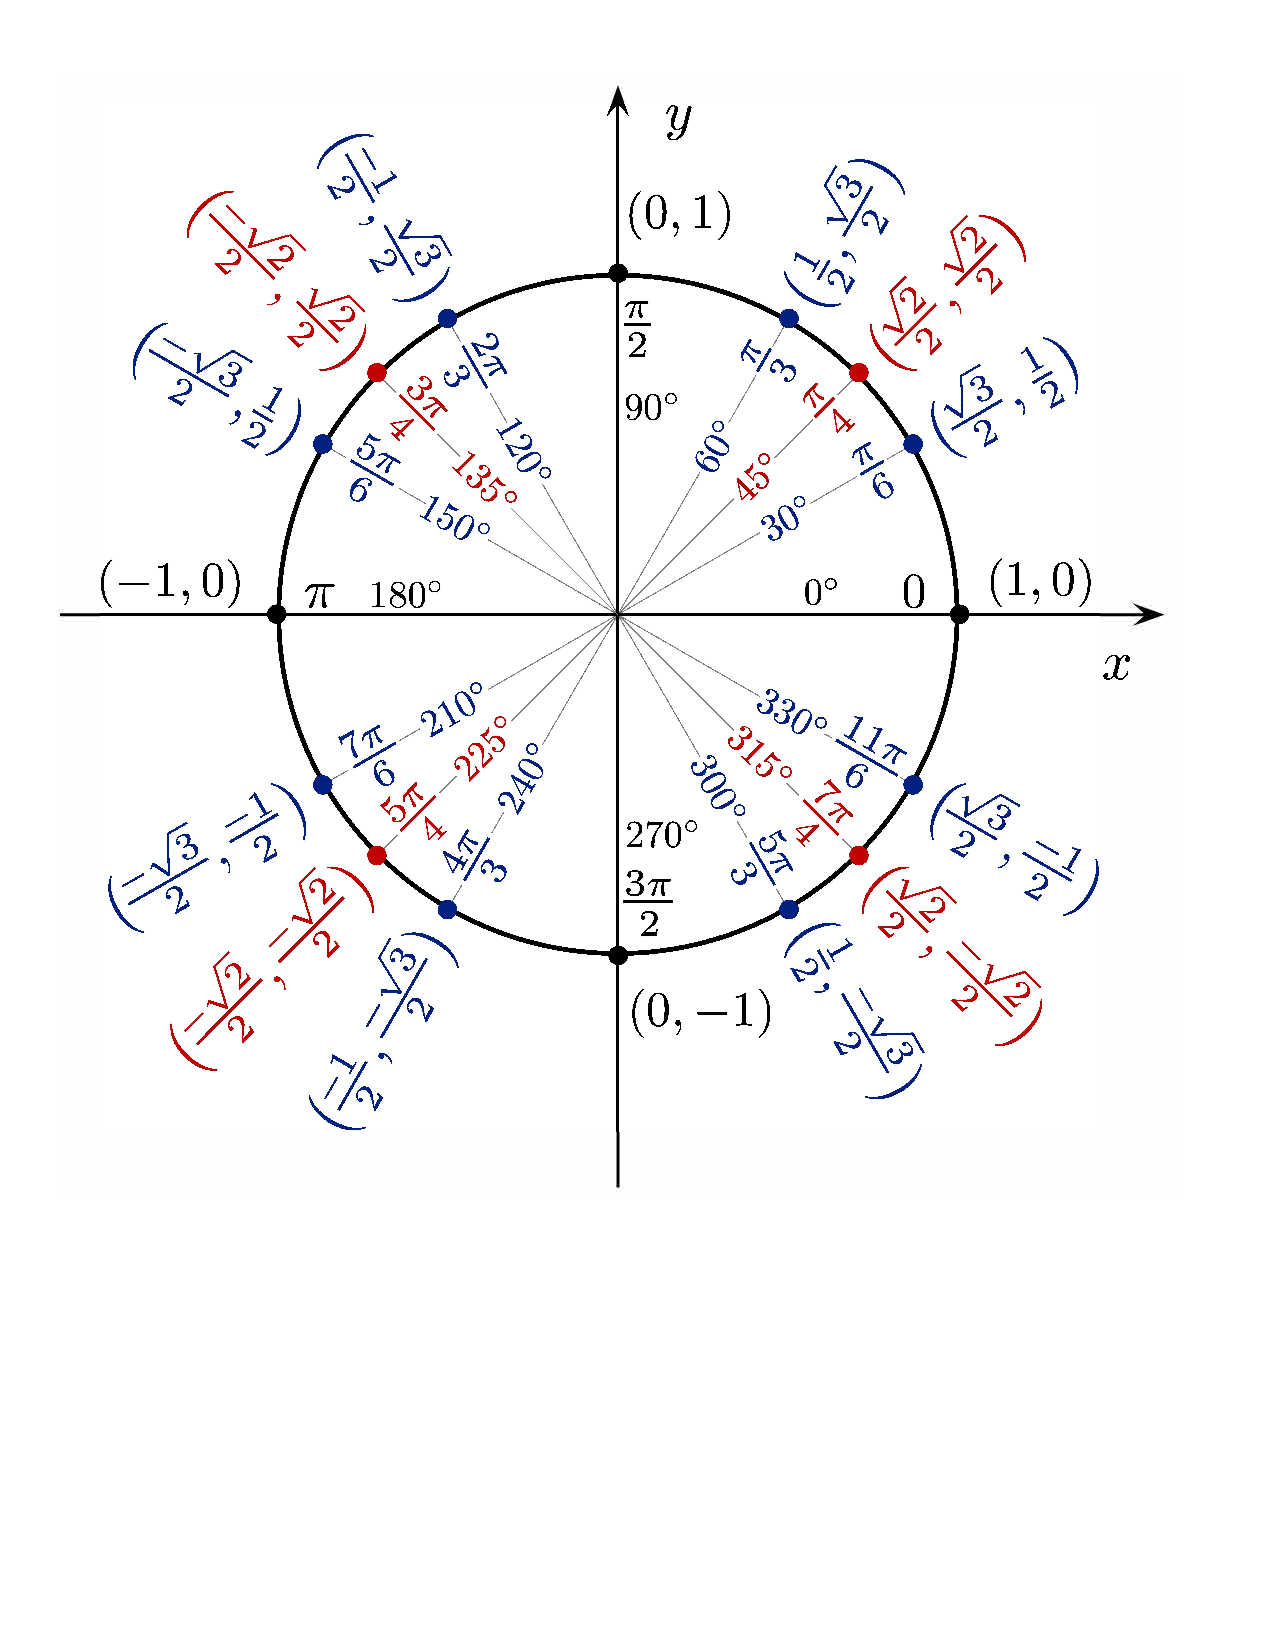
\includegraphics[width=2.25in]{../Images/ComplexNumbers/Unitcircledetailed}
  %\documentclass[%
%% border=1pt
%  border={0pt 0pt 0pt 0pt} % left bottom right top
%]{standalone}
%\usepackage{tikz} % Required for drawing custom shapes
%\usepackage{pgfplots}
%\pgfplotsset{compat = newest}
%
%\usepackage{amsbsy}
%\usetikzlibrary{decorations.pathreplacing,calc}
%\usetikzlibrary{shapes}
%\usepackage{amsmath,stackrel}
%\usetikzlibrary{arrows.meta}
%\usetikzlibrary{arrows}
%\usetikzlibrary{calc}
%\usetikzlibrary{math}
%
%\begin{document}
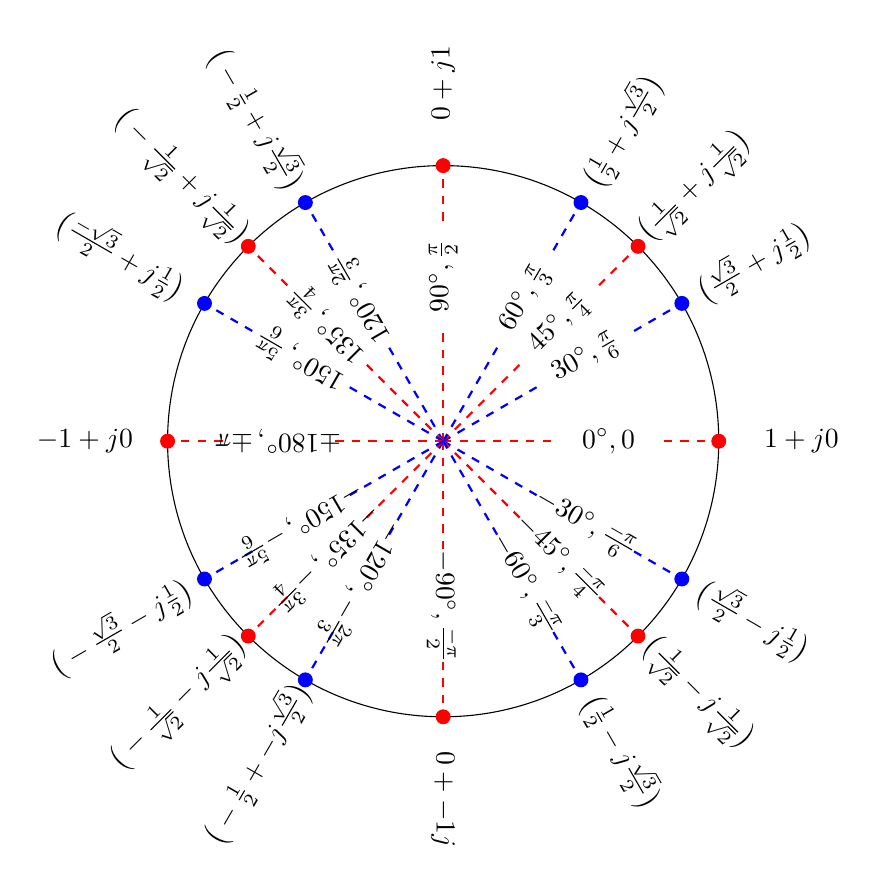
\begin{tikzpicture}[scale=0.7]
%\draw[style=help lines] (-12,-12) grid (12,12);
%\draw[black,->] (-12,0) -- (12,0);
%\draw[black,->] (0,-12) -- (0,12);

\draw (0,0) circle[radius=5];

\draw[fill,red] (0:5cm) circle[radius=0.125];
\draw[red,dashed,thick] (0,0) -- (0:2cm) (0:4cm) -- (0:5cm);
\node[rotate=0] at (0:3cm){$0^\circ, 0$};
\node at (0:6.5cm)[rotate=0]{$1+j0$};

\draw[fill,blue] (30:5cm) circle[radius=0.125];
\draw[blue,dashed,thick] (0,0) -- (30:2cm) (30:4cm) -- (30:5cm);
\node[rotate=30] at (30:3cm){$30^\circ, \frac{\pi}{6}$};
\node at (30:6.5cm)[rotate=30]{$\big(\frac{\sqrt{3}}{2}+j\frac{1}{2} \big)$};

\draw[fill,red] (45:5cm) circle[radius=0.125];
\draw[red,dashed,thick] (0,0) -- (45:2cm) (45:4cm) -- (45:5cm);
\node[rotate=45] at (45:3cm){$45^\circ, \frac{\pi}{4}$};
\node at (45:6.5cm)[rotate=45]{$\big(\frac{1}{\sqrt{2}}+j\frac{1}{\sqrt{2}} \big)$};

\draw[fill,blue] (60:5cm) circle[radius=0.125];
\draw[blue,dashed,thick] (0,0) -- (60:2cm) (60:4cm) -- (60:5cm);
\node[rotate=60] at (60:3cm){$60^\circ, \frac{\pi}{3}$};
\node at (60:6.5cm)[rotate=60]{$\big(\frac{1}{2}+j\frac{\sqrt{3}}{2} \big)$};

\draw[fill,red] (90:5cm) circle[radius=0.125];
\draw[red,dashed,thick] (0,0) -- (90:2cm) (90:4cm) -- (90:5cm);
\node[rotate=90] at (90:3cm){$90^\circ, \frac{\pi}{2}$};
\node at (90:6.5cm)[rotate=90]{$0+j1$};

\draw[fill,blue] (120:5cm) circle[radius=0.125];
\draw[blue,dashed,thick] (0,0) -- (120:2cm) (120:4cm) -- (120:5cm);
\node[rotate=120] at (120:3cm){$120^\circ, \frac{2\pi}{3}$};
\node at (120:6.75cm)[rotate=-60]{$\big(-\frac{1}{2}+j\frac{\sqrt{3}}{2} \big)$};

\draw[fill,red] (135:5cm) circle[radius=0.125];
\draw[red,dashed,thick] (0,0) -- (135:2cm) (135:4cm) -- (135:5cm);
\node[rotate=135] at (135:3cm){$135^\circ, \frac{3\pi}{4}$};
\node at (135:6.75cm)[rotate=-45]{$\big(-\frac{1}{\sqrt{2}}+j\frac{1}{\sqrt{2}} \big)$};

\draw[fill,blue] (150:5cm) circle[radius=0.125];
\draw[blue,dashed,thick] (0,0) -- (150:2cm) (150:4cm) -- (150:5cm);
\node[rotate=150] at (150:3cm){$150^\circ, \frac{5\pi}{6}$};
\node at (150:6.75cm)[rotate=-30]{$\big(\frac{-\sqrt{3}}{2}+j\frac{1}{2} \big)$};

R\draw[fill,red] (180:5cm) circle[radius=0.125];
\draw[red,dashed,thick] (0,0) -- (180:2cm) (180:4cm) -- (180:5cm);
\node[rotate=180] at (180:3cm){$\pm 180^\circ, \pm \pi$};
\node at (180:6.5cm)[rotate=0]{$-1+j0$};

\draw[fill,blue] (-30:5cm) circle[radius=0.125];
\draw[blue,dashed,thick] (0,0) -- (-30:2cm) (-30:4cm) -- (-30:5cm);
\node[rotate=-30] at (-30:3cm){$-30^\circ, \frac{-\pi}{6}$};
\node at (-30:6.5cm)[rotate=-30]{$\big(\frac{\sqrt{3}}{2}-j\frac{1}{2} \big)$};

\draw[fill,red] (-45:5cm) circle[radius=0.125];
\draw[red,dashed,thick] (0,0) -- (-45:2cm) (-45:4cm) -- (-45:5cm);
\node[rotate=-45] at (-45:3cm){$-45^\circ, \frac{-\pi}{4}$};
\node at (-45:6.5cm)[rotate=-45]{$\big(\frac{1}{\sqrt{2}}-j\frac{1}{\sqrt{2}} \big)$};

\draw[fill,blue] (-60:5cm) circle[radius=0.125];
\draw[blue,dashed,thick] (0,0) -- (-60:2cm) (-60:4cm) -- (-60:5cm);
\node[rotate=-60] at (-60:3cm){$-60^\circ, \frac{-\pi}{3}$};
\node at (-60:6.5cm)[rotate=-60]{$\big(\frac{1}{2}-j\frac{\sqrt{3}}{2} \big)$};

\draw[fill,red] (-90:5cm) circle[radius=0.125];
\draw[red,dashed,thick] (0,0) -- (-90:2cm) (-90:4cm) -- (-90:5cm);
\node[rotate=-90] at (-90:3cm){$-90^\circ, \frac{-\pi}{2}$};
\node at (-90:6.5cm)[rotate=-90]{$0+-1j$};

\draw[fill,blue] (-120:5cm) circle[radius=0.125];
\draw[blue,dashed,thick] (0,0) -- (-120:2cm) (-120:4cm) -- (-120:5cm);
\node[rotate=-120] at (-120:3cm){$-120^\circ, -\frac{2\pi}{3}$};
\node at (-120:6.75cm)[rotate=60]{$\big(-\frac{1}{2}+-j\frac{\sqrt{3}}{2} \big)$};

\draw[fill,red] (-135:5cm) circle[radius=0.125];
\draw[red,dashed,thick] (0,0) -- (-135:2cm) (-135:4cm) -- (-135:5cm);
\node[rotate=-135] at (-135:3cm){$-135^\circ, -\frac{3\pi}{4}$};
\node at (-135:6.75cm)[rotate=45]{$\big(-\frac{1}{\sqrt{2}}-j\frac{1}{\sqrt{2}} \big)$};

\draw[fill,blue] (-150:5cm) circle[radius=0.125];
\draw[blue,dashed,thick] (0,0) -- (-150:2cm) (-150:4cm) -- (-150:5cm);
\node[rotate=-150] at (-150:3cm){$-150^\circ,-\frac{5\pi}{6}$};
%\node[rotate=-150] at (-150:3.5cm){$-\frac{\pi}{6}$};
\node at (-150:6.75cm)[rotate=30]{$\big(-\frac{\sqrt{3}}{2}-j\frac{1}{2} \big)$};

\end{tikzpicture}
%\end{document} 
  \caption{Unit circle showing the Cartesian and polar representation of commonly encountered complex numbers}
  \label{fig:unitcircledetailed}
\end{figure}
%In Fig.~\ref{fig:unitcircledetailed}, the Cartesian form is given as two coordinates. For example, $\bigg(\frac{1}{2},\frac{\sqrt{3}}{2}\bigg)$ refers to the complex number
%$\frac{1}{2}+j \frac{\sqrt{3}}{2}$. Similarly, $(0,1)$ refers to the complex number is $0+j1 = j$.

\begin{example}
It is very useful to know the polar form for often used complex numbers such as $1,j,-j,-1$. They are given by
\[
\boxed{1 = e^{j0}, -1 = e^{j \pi}, j = e^{j \frac{\pi}{2}}, -j = e^{-j \frac{\pi}{2}}}.
\]
\end{example}

\begin{example}
Let $z = 2 e^{j \frac{\pi}{4}}$. Find the magnitude and angle of $z$. The answer is $|z|=2$ and $\theta = \pi/4$. Many students will first convert $z$ to Cartesian form, write it as $z = \sqrt{2} + j \sqrt{2}$ and then compute $|z|$ as $\sqrt{(\sqrt{2})^2+(\sqrt{2})^2}$. While this is not wrong, this is time consuming and misses the point. You should train yourself to see that $z$ is already given in polar form, i.e., as $r e^{j \theta}$ with $r = 2$ and $\theta = \pi/4$. Since $r$ represents the magnitude of $z$, you can directly read off the magnitude as 2 and angle as $\pi/4$. In my experience, students have difficulty with this sometimes well into the course.
\end{example}

\begin{example}
Let $z = -2 e^{j \frac{\pi}{4}}$. Find $|z|$ and $\angle z$.

The point of this example is to emphasize that the magnitude of a complex number $r$ must be positive.
It would be wrong to say that $|z| = -2$.
We must rewrite $z$ as $z = 2 e^{j \pi} e^{j \frac{\pi}{4}} = 2 e^{j \frac{5 \pi}{4}}$ and interpret $r$ as $2$ instead of $-2$ and the angle as $\pi + \pi/4 = 5 \pi/4$.
\end{example}

%As simple as this seems, I have repeatedly noticed students making mistakes in this.

Caution: The expression for $\theta$ in (\ref{eqn:magandphase}) does not identify $\theta$ uniquely, since $\tan(\theta) = \frac{y}{x}$ also implies
that $\tan(\theta \pm \pi) = \frac{y}{x}$. It is best think of the vector $(x,y)$ and determine which quadrant this vector
lies in based on the signs of $x,y$ and then make sure $\theta$ corresponds to an angle in the correct quadrant.


\begin{example}
Suppose $z_1 = \frac{\sqrt{3}}{2}+j\frac{1}{2}$ and $z_2 = -\frac{\sqrt{3}}{2}-j\frac{1}{2}$. It is easy to see that $\tan^{-1}\left(\frac{y_1}{x_1} \right)
= \tan^{-1}\left(\frac{y_2}{x_2} \right)$. However, $z_1$ is complex number in the first quadrant, whereas $z_2$ is a complex number in the 3rd quadrant. Therefore, $\theta_1$ should be $\pi/6$ and $\theta_2$ should be $7 \pi/6$.
\end{example}

\begin{infobox}{Periodicity of complex exponentials}
One important aspect of the polar form for a complex number is that adding $2 \pi$ to the angle does not change the complex number. Particularly,
\[
r e^{j\theta} = re^{j(\theta+2 k \pi)} \ \ \ \hbox{for any integer} \ k
\]
\end{infobox}
This fact will be repeatedly used in the course. An immediate example of where this is useful is given in Section~\ref{sec:nthroots}.


\begin{example}
Express $e^{j 2 \pi}, e^{-j \pi}, e^{j \frac{3 \pi}{2}}, e^{j \frac{9 \pi}{2}}, e^{j \pi}$ in Cartesian form.
\end{example}

\newpage

\section{Conjugate - (\href{https://youtu.be/Bhkp4Bs1SKg}{Video})}
The conjugate of a complex number $z = x + j y$ is given by
$z^* = x - j y$. When $z$ is written in polar form as $z = r e^{j \theta}$, the
complex conjugate is given by $z^* = r e^{-j \theta}$. In general, to compute the conjugate of a
complex number, replace $j$ by $-j$ everywhere.
\begin{figure}[hbt]
%\begin{center}\includegraphics[width=2.5in]{../Figures/complexconjugate.pdf}\end{center}
\begin{center}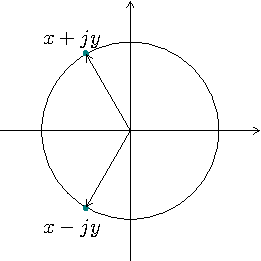
\includegraphics[width=2.5in]{../Images/ComplexNumbers/Fig_0_2.pdf}\end{center}
\caption{Conjugate of a complex number}
\label{fig:complexconjugate}
\end{figure}

\section{Arithmetic with two complex numbers - (\href{https://youtu.be/XFXuDNh4kOA}{Video})}
Let $z = x + j y = r e^{j \theta}$,  $z_1 = x_1 + j y_1 = r_1 e^{j \theta_1}$ and $z_2 = x_2 + j y_2  = r_2 e^{j \theta_2}$. 
We can perform arithmetic operations on complex numbers such as addition, subtraction, multiplication,
division, exponentiation (raising a complex number to powers) etc by treating $j$ as a real constant and
then simplifying or reducing the result using 
\[
j^2 = -1, \ j^3 = -j, \ j^4 = 1, \ j^5 = j, \ \ldots.
\]
The real and imaginary parts of the result of the computation are grouped and simplified together to yield 
a complex number in Cartesian form as the end result.  
While it is relatively easy to express the results of addition, subtraction, multiplication, and raising a complex number to integer powers in Cartesian form, a slightly more involved computation is required in order to express the result
of division in Cartesian form.
The following examples will make this more concrete

\begin{example}
Let $z_1 = 1+j$ and $z_2 = 2 + 3j$. Compute $z_1+z_2$, $z_1-z_2$, and $z_1 z_2$ and express the result in Cartesian form.

\begin{eqnarray*}
z_1 + z_2 & = & (1+j) + (2+3j) = (1+2) + (j+3j) = 3 + j(1+3) = 3 + 4j \\
z_1 - z_2 & = & (1+j) - (2+3j) = (1-2) + (j-3j) = -1 + j(1-3) = -1 -2j \\
z_1 z_2 & = & (1+j) (2+3j) = 1 \cdot 2 + 1 \cdot 3j +j \cdot 2 + j \cdot (3j) = 2 + 3j + 2j + 3\underbrace{j^2}_{=-1}\\
& = & (2-3) + j (3+2) = -1 + 5j
\end{eqnarray*}
\end{example}

A special case of multiplying two complex numbers is multiplying a complex number $z$ with its conjugate $z^*$.
We can see that $zz^*$ is given by
\[
zz^* = (x+jy)(x-jy) = x^2 +j yx - jxy -j^2y^2 = (x^2+y^2)+j(yx-xy) = x^2+y^2 = |z|^2.
\]
If the complex number is specified in polar form $z=re^{j\theta}$, then $zz^*$ can be computed as
\[
zz^* = r e^{j\theta} r e^{-j \theta} = r^2 e^{j \theta} e^{-j \theta} = r^2 = |z|^2.
\]
Therefore, multiplying $z$ by its conjugate, $z^*$ always results in $|z|^2$, which is a {\em real} number. 
This is a useful fact to keep in mind. 

\begin{example}
Let $z_1 = 1+j$ and $z_2 = 2 + 3j$. Compute $z_1/z_2$ and express the result in Cartesian form.

We begin by noticing that $\frac{z_1}{z_2} = \frac{1+j}{2+3j}$ and that it is not directly in Cartesian form.
To convert this to Cartesian form, we multiply the numerator and the denominator by the conjugate of $z_2$ yielding
\[
\frac{z_1}{z_2} = \frac{1+j}{2+3j} = \frac{(1+j)(2-3j)}{(2+3j)(2-3j)} = \frac{5-j}{2^2+3^2} = \frac{5}{13} - j \frac{1}{13}.
\]
\end{example}

If the complex numbers $z_1$ and $z_2$ are specified in polar form, i.e. $z_1 = r_1 e^{j \theta_1}$ and $z_1 = r_2 e^{j \theta_2}$, then in order to add or subtract complex numbers,
we should first convert them to Cartesian form and then add or subtract them in Cartesian form.
However, multiplying and dividing complex numbers is easier directly in polar form. 
\begin{eqnarray}
z_1 z_2 & = & r_1 e^{j \theta_1} r_2 e^{j \theta_2} = r_1 r_2 e^{j (\theta_1+\theta_2)} \\
\frac{z_1}{z_2} & = & \frac{r_1 e^{j \theta_1}}{r_2 e^{j \theta_2}} = 
\frac{r_1}{r_2} e^{j (\theta_1 - \theta_2)}.
\end{eqnarray}

\begin{infobox}{Arithmetic with complex numbers}
To summarize,
\begin{eqnarray}
\label{eqn:complexadd} z_1 \pm z_2 & = & (x_1 \pm x_2) + j (y_1 \pm y_2) \\
\label{eqn:complexmult} z_1 z_2 & = & (x_1 x_2 - y_1 y_2) + j (x_1 y_2 + x_2 y_1) = r_1 r_2 e^{j (\theta_1+\theta_2)} \\
\nonumber |z| &=& \sqrt{zz^*} = r\\
\nonumber \frac{z_1}{z_2} &=& \frac{(x_1+jy_1)}{(x_2+jy_2)} = \frac{(x_1+jy_1)(x_2-jy_2)}{x_2^2+y_2^2} = \frac{r_1}{r_2} e^{j (\theta_1-\theta_2)}
\end{eqnarray}
Typically, adding and subtracting complex numbers will be easier when the Cartesian form is used whereas, multiplication and division will be easier when the polar form is used. It will be important to be able to use both these representations in order to make computations easier.
\end{infobox}


\section{Geometric interpretation of arithmetic operations - (\href{https://youtu.be/A0j17Gg3JCM}{Video},
\href{https://colab.research.google.com/drive/1IPisKbolmXp2UD7ZuxIRhMEjvaq_Q82G?usp=sharing}{Python notebook})}
It is often useful to understand geometrically what we are doing when we are adding, subtracting, multiplying or dividing two complex numbers.
If we think of complex numbers are two-dimensional vectors, then adding and subtracting two complex numbers is the same as adding and subtracting vectors.
Standard geometrical interpretations such as the parallelogram method or tip-to-toe method are useful to gain visual insight.
However, multiplying and dividing vectors are typically not valid or well-defined operations.
Multiplying a complex number $z_1 = r_1 e^{j \theta_1}$ by $z_2 = r_2 ie^{j \theta_2}$ corresponds to doing two operations to $z_1$ - we scale the magnitude of $z_1$ by $r_2$ and then rotate the result by $\theta_2$ in the counter-clockwise direction.
Similarly, dividing $z_1$ by $z_2$ corresponds to scaling the magnitude of $z_1$ by $1/r_2$ and rotating the result by $\theta_2$ in the clockwise direction.
These are illustrated in Fig.~\ref{fig:geometricinterpretation}.

\begin{figure}[h]
  \centering
  %\documentclass[%
%% border=1pt
%  border={0pt 0pt 0pt 0pt} % left bottom right top
%]{standalone}
%\usepackage{tikz} % Required for drawing custom shapes
%\usepackage{pgfplots}
%\pgfplotsset{compat = newest}
%
%\usepackage{amsbsy}
%\usetikzlibrary{decorations.pathreplacing,calc}
%\usetikzlibrary{shapes}
%\usepackage{amsmath,stackrel}
%\usetikzlibrary{arrows.meta}
%\usetikzlibrary{arrows}
%\usetikzlibrary{calc}
%\usetikzlibrary{math}
%
%\begin{document}
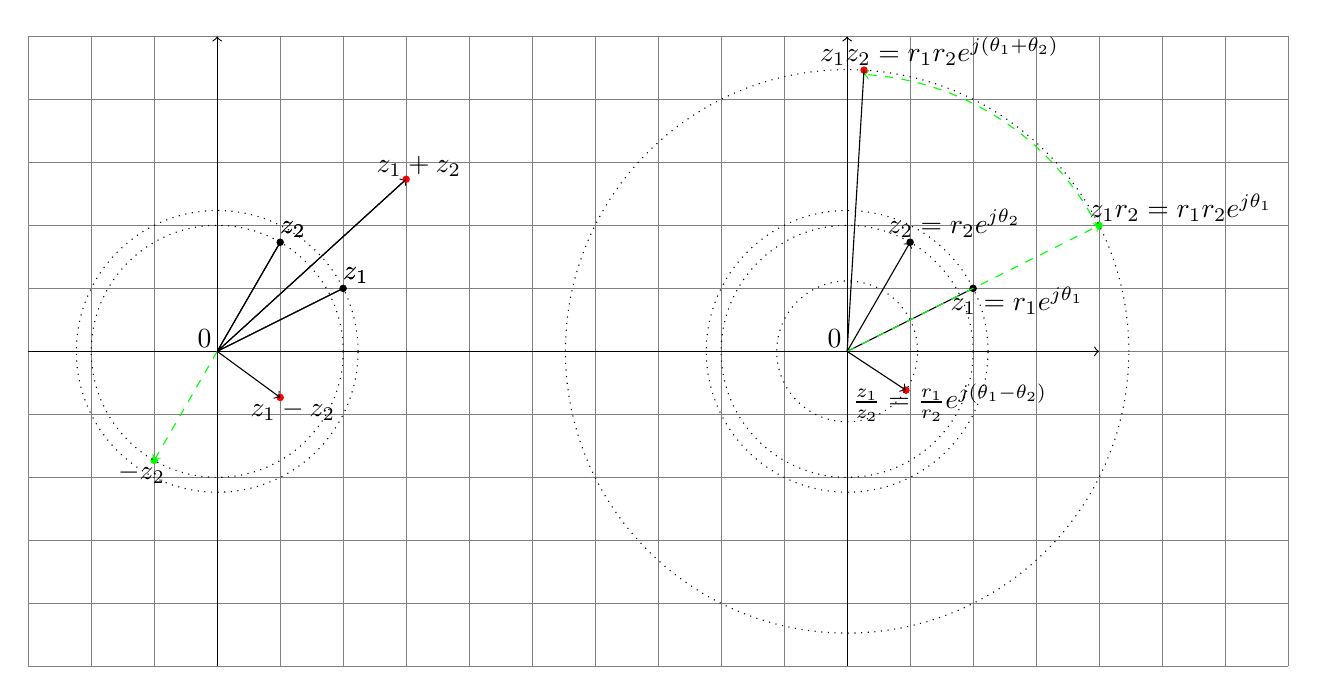
\begin{tikzpicture}[scale=0.8]
\draw[style=help lines] (-5,-5) grid (15,5);
\draw[black,->] (-5,0) -- (12,0);
\draw[black,->] (0-2,-5) -- (0-2,5);

\draw[fill] (2-2,1) circle[radius=0.05];
\draw[fill] (1-2,1.732) circle[radius=0.05];
\draw[fill,green] (-1-2,-1.732) circle[radius=0.05];
\node at (1.2-2,1.932) {$z_2$};
\node at (2.2-2,1.2) {$z_1$};
\node at (-1.2-2,-1.932) {$-z_2$};

\draw[->] (0-2,0) -- (2-2,1) (0-2,0) -- (1-2,1.732) (0-2,0) -- (3-2,2.732);
\draw[->,green,dashed] (0-2,0) -- (-1-2,-1.732);

\draw[fill,red] (3-2,2.732) circle[radius=0.05];
\draw[fill,red] (1-2,-0.732) circle[radius=0.05];

%\draw[fill,red] ({0.46*360/(2*pi)+60}:{2*sqrt(5)}) circle[radius=0.05];
%\draw[fill,red] ({0.46*360/(2*pi)-60}:{sqrt(5)/2}) circle[radius=0.05];

\draw[dotted] (0-2,0) circle[radius={sqrt(5)}];
\draw[dotted] (0-2,0) circle[radius=2];

\node at (1.2-2,1.932) {$z_2$};
\node at (2.2-2,1.2) {$z_1$};
\node at (3.2-2,2.932){$z_1+z_2$};
\node at (1.2-2,-0.932){$z_1-z_2$};
\draw[->] (0-2,0) -- (2-2,1) (0-2,0) -- (1-2,1.732) (0-2,0) -- (3-2,2.732) (0-2,0) -- (1-2,-0.732);
\node at (-0.2-2,0.2) {0};
%---------------------------------------------------------------------------------------------------
%\draw[black,->] (1,0) -- (10,0);
\draw[black,->] (8,-5) -- (8,5);

\draw[fill] (10,1) circle[radius=0.05];
\draw[fill] (9,1.732) circle[radius=0.05];
\draw[fill,green] (12,2) circle[radius=0.05];

\node at (9.2+0.5,1.932+0.1) {$z_2 = r_2 e^{j \theta_2}$};
\node at (10.2+0.5,1.2-0.4) {$z_1 = r_1 e^{j \theta_1}$};
\node at (12.2+1.1,1.932+0.35) {$z_1 r_2 = r_1 r_2 e^{j \theta_1}$};

\draw[->] (8,0) -- (10,1) (8,0) -- (9,1.732);
\draw[dashed,green,->] (8,0) -- (12,2);
%\draw[->] (26.5:{2*sqrt(5)}) arc (86.5:{2*sqrt(5)});
\draw[dashed,green,->] (12,1.932) arc[start angle=26.56505, end angle=60+26.56505,radius=4.472cm];

\draw[fill,red] (8.2679,4.4641) circle[radius=0.05];
\draw[fill,red] (8.9330,-0.6160) circle[radius=0.05];

%\draw[fill,red] ({0.46*360/(2*pi)+60}:{2*sqrt(5)}) circle[radius=0.05];
%\draw[fill,red] ({0.46*360/(2*pi)-60}:{sqrt(5)/2}) circle[radius=0.05];
\draw[dotted] (8,0) circle[radius=2];
\draw[dotted] (8,0) circle[radius={sqrt(5)}];
\draw[dotted] (8,0) circle[radius={2*sqrt(5)}];
\draw[dotted] (8,0) circle[radius={sqrt(5)/2}];

\node at (8.2679+1+0.2,4.4641+0.3){$z_1 z_2 = r_1 r_2 e^{j (\theta_1+\theta_2)}$};
\node at (8.9330+.2+0.5,-0.6160-0.2){$\frac{z_1}{z_2} = \frac{r_1}{r_2} e^{j (\theta_1 - \theta_2)}$};
\draw[->] (8,0) -- (8.2679,4.4641) (8,0) -- (8.9330,-0.6160);
\node at (8-0.2,0.2) {0};
\end{tikzpicture}
%\end{document} 
  \caption{What are we doing geometrically when we are adding, subtracting, multiplying and dividing complex numbers?
  Left panel show addition and subtraction of complex numbers. Right panel shows multiplication and division of complex numbers.
  $z_1 z_2$ is obtained by first scaling $z_1$ by $r_2$ and then rotating the result by $\theta_2$ counter-clockwise.}
  \label{fig:geometricinterpretation}
\end{figure}


\section{More properties of complex numbers}
The student should verify that these properties hold for complex numbers.
\begin{eqnarray}
\nonumber (z_1+z_2)^* & = & z_1^* + z_2^*\\
\nonumber (z_1 \ z_2)^* & = & z_1^* \ z_2^* \\
\nonumber \left(\frac{z_1}{z_2}\right)^* & = & \frac{z_1^*}{z_2^*} \\
\nonumber |z_1-z_2| &=& \sqrt{(x_1-x_2)^2+(y_1-y_2)^2}\\
\nonumber |z_1z_2| &=& |z_1||z_2| = r_1 r_2 \\
\nonumber \left|\frac{z_1}{z_2}\right| &=& \frac{|z_1|}{|z_2|} = \frac{r_1}{r_2}\\
\nonumber z z^* &=& x^2 + y^2 = r^2 = |z|^2\\
\nonumber z + z^* & = & 2 \Re\{z\} \\
\nonumber z - z^* & = & 2 j \Im \{z\}
\end{eqnarray}

\section{Fields, Fundamental theorem of algebra, and algebraic closure}
\label{sec:algebraicclosure}
We can add, subtract, multiply, and divide two complex numbers and the result will be another complex number. Further, there are identities for addition and multiplication of complex numbers, i.e.. $0+z = z$ and $(1+j0) z = z$ for any complex number $z$. For every complex number $z$,
there is another complex number $1/z$ which is the inverse of $z$. Formally, in mathematics, we call such a set of numbers with the associated addition and multiplication operations as a field. Thus complex numbers form a field, typically denoted by
$\mathbb{C}$.

There are many fields. For example, the set of real numbers with conventional addition and multiplication form a field, the set of rational numbers is also a field.
However, there is something special about the field of complex numbers.
The \href{https://en.wikipedia.org/wiki/Fundamental_theorem_of_algebra}{fundamental theorem of algebra} states that every non-zero, single-variable, degree-$n$ polynomial with complex coefficients has, counted with multiplicity, exactly $n$ complex roots.
Such a statement is not true for real numbers or rational numbers. For example,
$x^2+1 = 0$ is polynomial equation with real coefficients; but it's roots are not real.
However, with complex numbers, we are guaranteed that every degree-$n$ equation has roots
within the complex field. Because of this, we say that complex numbers are algebraically closed. \href{https://www.youtube.com/watch?v=shEk8sz1oOw}{Numberphile's video on the fundamental theorem of algebra} has more details.

The fact that we can add, subtract, multiply, divide, invert complex numbers and solve equations with coefficients and stay within the complex field makes the complex number system quite rich in what we can do with complex numbers. Hence, it is used a lot in mathematics and engineering.


\section{$n^{th}$ power of a complex number - (\href{https://youtu.be/um6i6G5WaU8}{Video 1})}
\label{sec:nthpower}

Let $z_0 = x_0 + j y_0 = r_0  e^{j \theta_0}$. For any integer $n$, the $n$th power of $z$, $z^n$ is simply obtained by
using (\ref{eqn:complexmult}) $n$ times. In the polar form, $z_0^n = r_0^n e^{j n \theta_0}$. Just like how the two real
numbers $1$ and $-1$ have the same square, different complex numbers can have the same $n$th power.

Consider the set of distinct complex numbers $z_k = e^{j \theta_0 + \frac{2 \pi (k-1)}{n}}$. All the $z_k$s are different have the same $n$th power for $k=1,2,\ldots,n$. We can see this by raising $z_k$ to the $n$th power to get
\begin{equation}
z_k^n = \left(e^{j \theta_0 + \frac{2 \pi (k-1)}{n}}\right)^n = e^{j n \theta_0 + 2 \pi (k-1)} = e^{j n \theta_0}.
\end{equation}

\section{$n^{th}$ roots of a complex number -
(\href{https://youtu.be/MOudd6zG72Q}{Video 1},
\href{https://youtu.be/DKW7Fkvb4JA}{Video 2},
\href{https://colab.research.google.com/drive/1SQh4WxEiAz03-S8pS9OXiNRmV2Go5bRh?usp=sharing}{Python notebook})}
\label{sec:nthroots}
The $n$th root of $z_0$ is a bit more interesting and tricky. Any complex number $z$ which is the solution to the $n$th degree equation
\[
z^n - z_0 = 0
\]
is an $n$th root of $z_0$. The fundamental theorem of algebra states that an $n$th degree equation has exactly $n$ (possibly complex and possibly repeated) roots. Hence, every complex number $z_0$ has exactly $n$, $n$th roots.  Let $z_1,z_2,\ldots,z_n$ denote the $n$ roots.
These roots can be found using
the fact $e^{j \theta} = e^{j (\theta + 2 \pi k)}$.
The $k$th root $z_k = r_k e^{j \theta_k}$ can be found by setting
\begin{eqnarray}
\nonumber
z_k^n = z_0 & \Rightarrow & r_k^n e_k^{jn\theta} = r_0 e^{j\theta_0} = r_0 e^{j(\theta_0 +2 k \pi)} \\
\label{eq:nthroot}
& \Rightarrow & r_k = \sqrt[n]{r_0}, \ \ \theta_k = \frac{\theta_0+2 \pi (k-1)}{n} \mbox{ for } k = 1,2,\ldots n
\end{eqnarray}
Here $\sqrt[n]{r_0}$ refers to the positive $n$th root.
Note that for all the $k$ roots, the magnitude is the same whereas the angles are different.
Clearly, computing $n$th roots is much easier in the polar form than in the Cartesian form.

\begin{example}

Find the third roots of unity $\sqrt[3]{1}$

Since $1 = 1 e^{j0}$, this corresponds to $r_0 = 1, \theta_0 = 0$. Hence, the three roots
of unity are given by
\[
r = 1, \ \ \theta = 0,\frac{2\pi}{3},\frac{4\pi}{3}.
\]

In cartesian coordinates, they are $(1+j0)$, $\left(-\frac{1}{2}+j\frac{\sqrt{3}}{2}\right)$, $\left(-\frac{1}{2}-j\frac{\sqrt{3}}{2}\right)$. These are referred to as $1,\omega,\omega^2$ sometimes. The three roots are shown in Figure~\ref{fig:cuberootsofunity}.
\begin{figure}[ht]
%\begin{center}\includegraphics{../Figures/cuberootsofunity.pdf}\end{center}
\begin{center}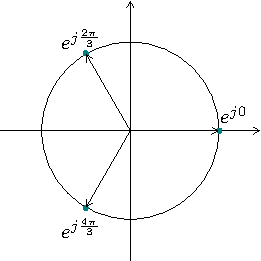
\includegraphics{../Images/ComplexNumbers/Chap0_cuberootsofunity.pdf}\end{center}
\caption{Cube roots of unity}
\label{fig:cuberootsofunity}
\end{figure}

\end{example}

\section{Functions of a complex variable - (\href{https://youtu.be/vxPfRFOrAyg}{Video})}

Let $f(z)$ be a complex function of a complex variable $z$, i.e., for every $z$, $f(z)$ is a complex number. Note that
a real number is also considered as a complex number and, hence, $f(z)$ could have a zero imaginary part. Examples of
functions include $f(z) = |z|, f(z) = \mbox{arg}(z), f(z) = z^n, f(z) = \exp(z)$, etc.
The exponential functions can be  interpreted using Euler's identity as follows.
\[
f(z) = \exp(z) = e^xe^{jy} = e^x\cos y + je^x\sin y
\]
%The real part of $f(z)$ is plotted as a function of the real part of $z$, namely $x$ for the case $x<0$ in Fig.~\ref{fig:realpartofexp}.
%\begin{figure}[ht]
%\begin{center}
%%\includegraphics{../Figures/3.pdf}
%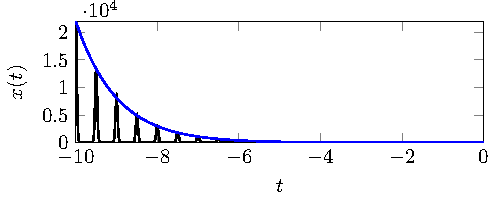
\includegraphics[width=4.0in]{../Images/ComplexNumbers/Chap0_realexpzversusrealz.pdf}
%\end{center}
%\caption{$\Re\{\exp{z}\}$ vs $\Re\{z\}$ and $\Re\{\exp{z}\}$ vs $\Im \{z\}$}
%\label{fig:realpartofexp}
%\end{figure}
The logarithm of a complex number $\ln z$ can be also interpreted using Euler's identity as
\[
\ln(z) = \ln\left(r e^{j (\theta + 2 k \pi) } \right) = \ln r + j (\theta + 2 k \pi).
\]
It can be seen from the above expression that $\ln z$ is not a function (i.e., there are many possible values of $\ln z$ for a given value of $iz$). However, if we set $k=0$ in the above expression, then we get what is called the principal value of $\ln z$, denoted by Ln $z$, which is a function.

Similarly, it is important to realize that for any integer $n$, the $n$th power of a complex number is a function of the complex number, i.e., for every complex number $z$, there is only one complex number $z^n$. However, for an integer $n$, the $n$th root of a complex number is not uniquely defined and hence, is not a function. Often, one may take the root corresponding to $k=0$ in (\ref{eq:nthroot}) as the default root and hence the principal value. Then, the principal value becomes a function. This is similar to square roots of positive real numbers being defined as the positive numbers. There are interesting examples where careless use of just the principal value as the $n$th root can lead to fallacious arguments.

\section{Complex functions of a real variable - (\href{https://youtu.be/jSsg4Pxib6o}{Video},
\href{https://colab.research.google.com/drive/1WvHOa8tOM4J4GjCw-zXwvfFW08QikVXb?usp=sharing}{Python notebook})}

You may be used to dealing with functions of a variable such as $y = f(x)$, where $x$ is called the independent variable and
$y$ is called the dependent variable and typically, $y$ takes real values when $x$ takes real values. In this course, we will be interested in complex functions of a real variable. Often the real variable will represent time or frequency. Such a function, normally denoted as $x(t)$ or $X(\omega)$ is a function which takes a complex value for every real value of the independent variable $t$ or $\omega$. Pay attention to the notation carefully - $t$ or $\omega$ now becomes the independent variable and $x(t)$ or $X(\omega)$ now becomes the dependent variable. We can also think of the complex function as the combination of two real functions of the independent variable, one for the real part of $x(t)$ and one for the imaginary part of $x(t)$.

When dealing with real functions of a real variable, you may be used to plotting the function $x(t)$ as a function of $t$. However, when $x(t)$ is a complex function, there is a problem in plotting this function since for every value of $t$, we need to plot a complex number. In this case, we do one of two things - either we plot the real part of $x(t)$ versus $t$ and plot the imaginary part of $x(t)$ versus t, or we plot $|x(t)|$ versus $t$ and $\mbox{arg}(x(t))$ versus $t$. Either of these is fine, but we do need two plots to effectively understand how $x(t)$ changes with $t$.

%-------------------------------
\begin{example} Consider the function  $x(t) = e^{j2\pi t} = \cos {2\pi t} +  j \sin {2\pi t}$ for all real values of $t$.
This is clearly a complex function of a real variable $t$. $\Re\{x(t)\}, \Im\{x(t)\}, |x(t)|, \mbox{arg}(x(t))$ are all real functions of the real variable $t$. Hence, we can plot $\Re\{x(t)\}$ versus $t$ and $\Im\{x(t)\}$ versus $t$ or we can plot $|x(t)|$ versus $t$ and $\angle x(t)$ versus $t$ as shown in Fig.~\ref{fig:x(t)example1}
\begin{figure}[hbtp]
\begin{center}
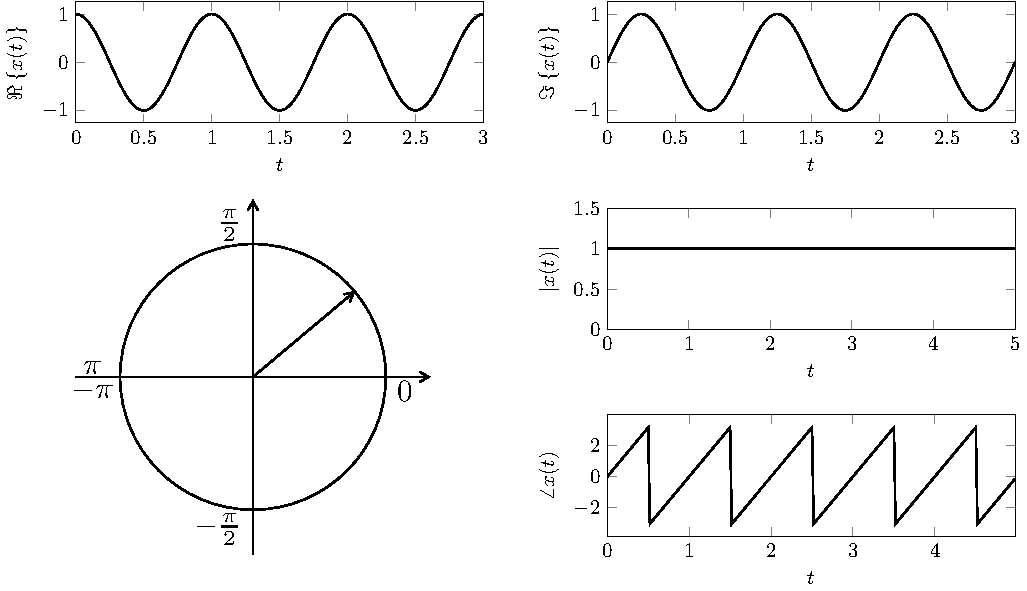
\includegraphics[width=6.0in]{../Images/ComplexNumbers/Fig_0_4.pdf}
%%\documentclass[%
%% border=1pt
%  border={0pt 0pt 0pt 0pt} % left bottom right top
%]{standalone}
%\usepackage{tikz} % Required for drawing custom shapes
%\usepackage{pgfplots}
%\pgfplotsset{compat = newest}
%
%\usepackage{amsbsy}
%\usetikzlibrary{decorations.pathreplacing,calc}
%\usetikzlibrary{shapes}
%\usepackage{amsmath,stackrel}
%\usetikzlibrary{arrows.meta}
%\usetikzlibrary{arrows}
%\usetikzlibrary{calc}
%\usetikzlibrary{math}
%
\begin{document}
\tikz{
%\begin{axis}[]
	\begin{axis}[enlarge x limits=0,
		enlarge y limits=0.13,
			xlabel={$t$},
		ylabel={$\Re \left\{x(t)\right\}$},
			width = 0.7\textwidth,
		height = 0.3\textwidth, ]
	\addplot[trig format =rad,black,domain=0:3,samples=200,thick]{cos(2*pi*x)}; % plot of real part of figure1.4
	%\addplot[black,domain=0:3,samples=200,thick]{sin(2*180*x)}; % plot of imaginary part of figure 1.4
	%\addplot[black,domain=0:10,samples=200,thick]{sqrt((cos(2*pi*x))^2+(sin(2*pi*x))^2)}; % plot of magnitude of figure 1.4
		%\addplot[black,domain=0:5,samples=2000,thick]{atan((tan(2*pi*x))}; % plot of angle of x of figure 1.4
	%\addplot[black,domain=0:10,samples=200,thick]{exp{-x}};
\end{axis}

	\begin{axis}[enlarge x limits=0,
		enlarge y limits=0.13,xshift=9cm,
			xlabel={$t$},
		ylabel={$\Im \left\{x(t)\right\}$},width = 0.7\textwidth,
		height = 0.3\textwidth,]
	\addplot[trig format =rad,black,domain=0:3,samples=200,thick]{sin(2*pi*x)}; % plot of imaginary part of figure 1.4

\end{axis}


\begin{axis}[enlargelimits=false,
	xshift=9cm,yshift=-3.5cm,ymin=0, ymax=1.5,
		xlabel={$t$},
	ylabel={$|x(t)|$},
	width = 0.7\textwidth,
	height = 0.3\textwidth,]
\addplot[trig format =rad,black,domain=0:5,samples=200,thick]{sqrt((cos(2*pi*x))^2+(sin(2*pi*x))^2)}; % plot of magnitude of figure 1.4

\end{axis}

\begin{axis}[enlarge x limits=0,
	enlarge y limits=0.13,xshift=9cm,yshift=-7cm,
	xlabel={$t$},
	ylabel={$\angle x(t)$},
	width = 0.7\textwidth,
	height = 0.3\textwidth,
	]
	%\addplot[trig format =rad,black,domain=0:5,samples=2000,thick]{atan((tan(2*pi*x))}; % plot of angle of x of figure 1.4
	\addplot[black,thick]
    table[col sep=comma]{Data_0_4.csv}; % plot of angle of x of figure 1.4
	
\end{axis}

\def\circ#1#2{
	\begin{scope}[shift={#1}, rotate=#2,scale=1.5,every node/.append style={transform shape}]
		\node[thick,circle,draw=black,minimum size=3cm] (A) at (0,0) {};
		\draw[thick,-{angle 60},black] (-2,0)--(2,0);
		\draw[thick,-{angle 60},black] (0,-2)--(0,2);
		\node[thick,below,inner sep=0.03cm,xshift=0.2cm] at (A.0) {$0$};
		\draw[thick,-{angle 60},black,rotate around={40:(0,0)}] (0,0)-- node[above,xshift=1cm]{} (1.5,0);
		\node[left,inner sep=0.03cm,xshift=-0.1cm,yshift=0.2cm] at (A.90) {$\frac{\pi}{2}$};
		\node[left,inner sep=0.03cm,xshift=-0.1cm,yshift=-0.2cm] at (A.270) {$-\frac{\pi}{2}$};
		\node[below,inner sep=0.03cm,xshift=-0.3cm,yshift=-0cm] at (A.180) {$-\pi$};
		\node[above,inner sep=0.03cm,xshift=-0.3cm,yshift=-0cm] at (A.180) {$\pi$};

	\end{scope}
}

\circ{(3,-4.3)}{0}

}
%\end{document}

\end{center}
\caption{Plot of $\Re\{x(t)\}, \Im\{x(t)\}, |x(t)|, \angle x(t)$ versus $t$ for $x(t) = e^{j 2 \pi t}$.}
\label{fig:x(t)example1}
\end{figure}
\end{example}

%--------------------------------
\begin{example}
Consider the function $x(t) = e^{st}$ where $s = \sigma + j \omega$ is some complex number. This is a complex function of a real variable $t$. The real part and imaginary part of $x(t)$ are each real functions of a real variable $t$ and can be obtained as follows. Notice that $x(t)$ can be written as
\begin{eqnarray*}
% \nonumber % Remove numbering (before each equation)
  x(t) &=& e^{\sigma+j\omega}t = e^{\sigma t} e^{j \omega t} \\
   &=& e^{\sigma t} \left(\cos(\omega t) + j \sin(\omega t) \right) \\
   &=& \underbrace{e^{\sigma t} \cos(\omega t)}_{\text{Real part}} + j \underbrace{e^{\sigma t} \sin(\omega t)}_{\text{imaginary part}}
\end{eqnarray*}
\begin{figure}[htbp]
\begin{center}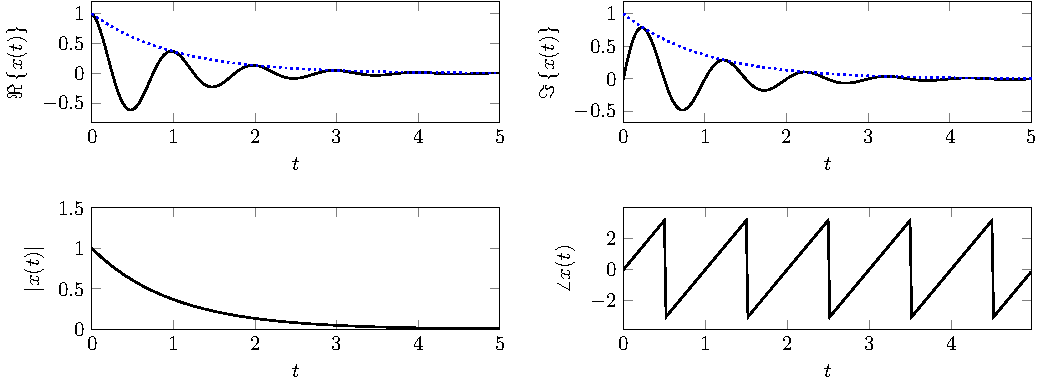
\includegraphics[width=6.0in]{../Images/ComplexNumbers/Fig_complexexponential.pdf}\end{center}
\caption{Plots of $\Re{x(t)}$ and $\Im{x(t)}$ versus $t$ and $|x(t)|$ and $\angle x(t)$ versus $t$.}
\label{fig:complexexponential}
\end{figure}
\end{example}
The magnitude of $x(t)$ and phase of $x(t)$ are both functions of $t$ given by
\begin{eqnarray*}
% \nonumber % Remove numbering (before each equation)
  |x(t)| &=& e^{\sigma t} \\
  \angle x(t) &=& \omega t
\end{eqnarray*}

These are plotted in Fig.~\ref{fig:complexexponential} for $\sigma = -1$ and $\omega = 2 \pi$.
The dotted blue lines in the figures show $|x(t)|$ and it can be seen that it defines the envelope of the real and imaginary
parts of $x(t)$.

It is useful to get insight into what happens to $x(t) = e^{st}$ as $t \rightarrow \infty$.
It can be seen that if $\sigma < 0$, $x(t) \rightarrow 0$ as $t \rightarrow \infty$ and if $\sigma > 0$, $x(t)$ becomes undefined at $t \rightarrow \infty$ with the $|x(t)| \rightarrow \infty$ as $t \rightarrow \infty$.
Thus, the real part of $s$ determines whether the function $x(t)$ is bounded or unbounded as $t \rightarrow \infty$.
%------------------------------

\begin{example} Consider the function $H(\omega) = \frac{1}{1+j\omega}$, where $\omega$ is a real variable.  Roughly sketch the magnitude and phase of $H(\omega)$ as a function of $\omega$.
\begin{eqnarray}
\nonumber H(\omega) &=& \frac{1}{1+j\omega}\\
\nonumber |H(\omega)| &=& \frac{1}{\sqrt{1+\omega^2}}\\
\nonumber \angle(H(\omega)) &=& 0-\tan^{-1}\omega
\end{eqnarray}

A plot of $|H(\omega)|$ versus $\omega$ and $\angle(H(\omega))$ versus $\omega$ is shown in Fig.~\ref{fig:Homegaexample1}.
\begin{figure}[htbp]
\begin{center}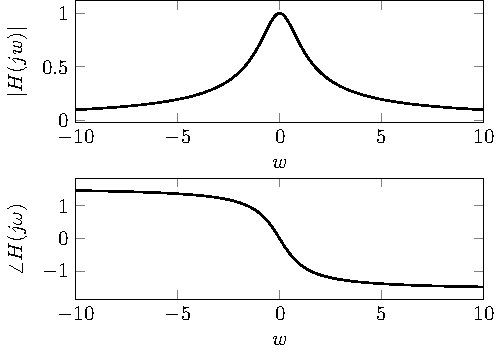
\includegraphics{../Images/ComplexNumbers/Fig_0_6.pdf}\end{center}
\caption{Plot of $H(\omega)$ vs $\omega$ and $\angle H(\omega)$ versus $\omega$ for $H(\omega) = \frac{1}{1+j\omega}$.}
\label{fig:Homegaexample1}
\end{figure}
\end{example}

\begin{example} Consider the function $X(\omega) = \frac{j \omega}{1+j\omega}$, where $\omega$ is a real variable.  Roughly sketch the magnitude and phase of $X(\omega)$ as a function of $\omega$.
\begin{eqnarray}
\nonumber X(\omega) &=& \frac{j\omega}{1+j\omega}\\
\nonumber |X(\omega)| &=& \frac{|\omega|}{\sqrt{1+\omega^2}}\\
\nonumber \angle(X(\omega)) &=& \left\{\begin{array}{ll}
-\frac{\pi}{2}-\tan^{-1}\omega &,\omega <0 \\
\frac{\pi}{2}-\tan^{-1}\omega &,\omega >0\end{array}
\right.
\end{eqnarray}

A plot of $|X(\omega)|$ versus $\omega$ and $\angle(X(\omega))$ versus $\omega$ is shown in Fig.~\ref{fig:Xomegaexample2}
\begin{figure}[htbp]
%\begin{center}\includegraphics{../Figures/4.pdf}\end{center}
\begin{center}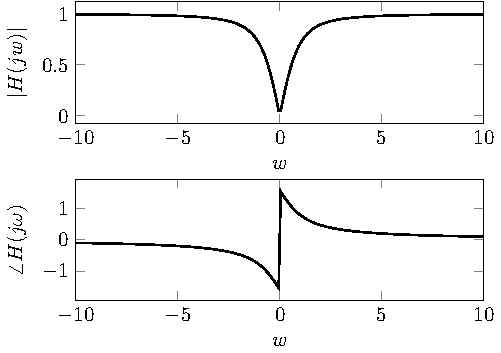
\includegraphics{../Images/ComplexNumbers/Fig_0_7.pdf}\end{center}
\caption{Plot of $X(\omega)$ vs $\omega$ and $\angle X(\omega)$ versus $\omega$ for $X(\omega) = \frac{j \omega}{1+j\omega}$.}
\label{fig:Xomegaexample2}
\end{figure}
\end{example}

\section{Plotting the magnitude and phase of $H(\omega) = e^{j a_1 \omega} + e^{j a_2 \omega}$ vs $\omega$ - (\href{https://youtu.be/Vse3mWToWc4}{Video})}
One of the tricks that is useful to get some insight into plotting the magnitude and phase of functions of the form $H(j \omega) = e^{j a_1 \omega} + e^{j a_2 \omega}$ vs $\omega$ is to express $e^{j a_1 \omega} + e^{j a_2 \omega}$ as follows
\begin{eqnarray}
\label{eq:sumofsinusoids}
e^{j a_1 \omega} + e^{j a_2 \omega} & = & e^{j \left(\frac{a_1+a_2}{2} \omega \right)} \left[ e^{j \left(\frac{a_1-a_2}{2} \right)\omega} + e^{-j \left( \frac{a_1-a_2}{2}\right) \omega } \right] \\
\nonumber
& = & e^{j \left(\frac{a_1+a_2}{2} \omega \right)} 2 \cos \left[ \left( \frac{a_1 - a_2}{2} \right) \omega \right]
\end{eqnarray}

Now, it is easy to see that $|H(\omega)| = 2 \left| e^{j \left(\frac{a_1+a_2}{2} \omega \right)}\right| \cdot \left| \cos \left[ \left( \frac{a_1 - a_2}{2} \right) \omega \right] \right| $ which is simply $2 \left| \cos \left[ \left( \frac{a_1 - a_2}{2} \right) \omega \right] \right|$.

\begin{example}
Compute the magnitude and phase of $H(\omega) = e^{j \omega} + e^{j 3 \omega}$ and determine the values of $\omega$ for which $H(\omega) = 0$.

\begin{eqnarray}
% \nonumber % Remove numbering (before each equation)
  H(\omega) = e^{j \omega} + e^{j 3 \omega} &=& e^{j 2 \omega} \left(e^{-j \omega} + e^{j \omega} \right) \\
  |H(\omega)| &=& 2 \cos \left( \omega \right) \\
  \angle H(\omega) &=& 2 \omega \ \text{sign}(\cos \omega)
\end{eqnarray}
\end{example}
\begin{figure}[htbp]
%\begin{center}\includegraphics{../Figures/4.pdf}\end{center}
\begin{center}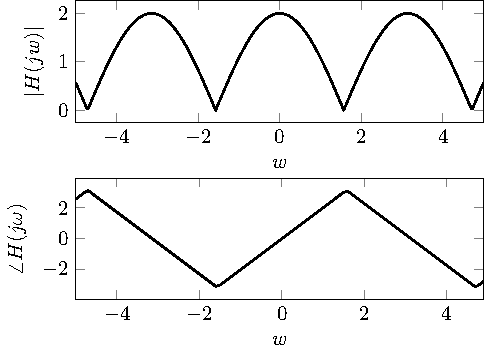
\includegraphics{../Images/ComplexNumbers/Fig_0_8.pdf}\end{center}
\caption{Plot of $|H(j \omega)|$ vs $\omega$ and $\angle H(j \omega)$ versus $\omega$ for $H(j \omega) = H(j \omega) = e^{j \omega} + e^{j 3 \omega}$.}
\label{fig:Xomegaexample3}
\end{figure}

The advantage computing the magnitude in this way lies in making it easy to compute values of $\omega$ for which $H(\omega)=0$.
The values of $\omega$ for which $|H(\omega)|=0$ which are simply given by the values of $\omega$ for which $2 \cos(\omega) = 0$. These are given by odd multiples of $\pi/2$, i.e., $\omega = (2i+1) \pi/2$ for any integer $i$.

\newpage

\section{Integrals of complex functions and integration by Parts -
(\href{https://youtu.be/CnbOzrYMJZE}{Video 1},
\href{https://youtu.be/4ltOPFdEeDY}{Video 2},
\href{https://colab.research.google.com/drive/1xX4C8epyw96KdPEsHzp1Xrq34HPCaIm4?usp=sharing}{Python notebook})}
In this class, we will encounter integrals of complex functions of a real variable integrated with respect to the real variable.
Let $x(t) = x_R(t)+jx_I(t)$ be a complex function of a real variable $t$.
The integral can be evaluated as the sum of $x_R(t)$ and $j x_I(t)$, where $x_R(t)$ and $x_I(t)$ are real functions of a real variable. The following result is true
\begin{equation}\label{eqn:integralcomplexfunctionofarealvariable1}
  \int_{a}^{b} x(t) \ dt = \int_{a}^{b} x_R(t) \ dt + j \int_{a}^{b} x_I(t) \ dt
\end{equation}
However, this approach will be very cumbersome in many cases as it will not be easy to split the integral into real and imaginary parts separately.
It will be easier to directly integrate the complex function.
All the rules of integration of real functions of real variables apply directly and $j$ can simply be treated as a constant.
In this class, we are typically interested in time $t$ or frequency $\omega$ being the independent variable.
Hence, the integrals will be with respect to $t$ or $\omega$.

For example,

\begin{example} Evaluate $\displaystyle{\int_0^{\pi/4} e^{j 2 t} \ dt}$

\[
\displaystyle{
\int_0^{\pi/4} e^{j 2 t} \ dt = \left[\frac{e^{j 2 t}}{2 j}\right]_{0}^{\pi/4} = \frac{j-1}{2j}
}
\]
\end{example}


\begin{example}
Evaluate $\displaystyle{\int_0^\infty e^{(-2+j3\pi)t} \ dt} $

\begin{eqnarray*}
% \nonumber % Remove numbering (before each equation)
  \displaystyle{\int_0^\infty e^{(-2+j3\pi)t} \ dt}  &=& \left[ \frac{e^{(-2+j3\pi)t}}{-2+j3} \right]_{0}^{\infty} \\
   &=& 0 - \frac{1}{-2+j3} = \frac{1}{2-j3}
\end{eqnarray*}
\end{example}

Sometimes we will have to use Integration by parts to evaluate integrals. The main result to recall is
\begin{equation}
\label{eq:byparts}
\displaystyle{\int_a^b u(t) \ dv(t) \ dt = \left[ u(t) \ v(t) \right]_a^b - \int_a^b v(t) \ du(t) \ dt}
\end{equation}

\begin{example}
Evaluate $\displaystyle{\int_0^1 t e^{-j \omega t} dt}$. Your answer should clearly be a function of $\omega$
\end{example}

We choose
\begin{eqnarray}
\nonumber
u(t) = t &,& dv(t) = e^{-j \omega t} \ dt \\
\nonumber
\Longrightarrow du(t)=dt &,&  v(t) = \frac{e^{-j \omega t}}{-j \omega}
\end{eqnarray}

\begin{eqnarray}
\nonumber
\int_0^1 t e^{-j \omega t} dt  & = & \displaystyle{\left[\frac{t e^{-j \omega t}}{-j \omega}\right]_0^1 - \int_0^1 \frac{e^{-j \omega t}}{-j \omega} \ dt}\\
\nonumber
& = & - e^{-j \omega} - \displaystyle{\left[\frac{e^{-j \omega t}}{-\omega^2} \right]_0^1} = - e^{-j \omega} +
\frac{e^{-j \omega}-1}{\omega^2}
\end{eqnarray}

In some cases, when we need to evaluate $\int x_R(t) \ dt$ or $\int x_I(t) \ dt$, it may be easier to think of an $x(t)$ whose real part is $x_R(t)$ or imaginary part is $x_I(t)$ and to integrate $x(t)$ first and then take the real part or the imaginary part.
We can then make use of the fact that in \eqref{eqn:integralcomplexfunctionofarealvariable1},
\begin{hintbox}{Integral of the real (imaginary) part is the real (imaginary) part of the integral}
\begin{eqnarray*}
\int x_R(t) \ dt  & = & \Re \left\{ \int x(t) \ dt \right\} \\
\int x_I(t) \ dt  & = & \Im \left\{ \int x(t) \ dt \right\}
\end{eqnarray*}
\end{hintbox}

The following example will highlight this
\begin{example}
Suppose we want to evaluate $\int e^{-at} \cos(bt) \ dt $ where $a$ and $b$ are real numbers.

One way to evaluate this integral is to apply integration by parts. There is an easier way using complex functions.
From Euler's identity, we know that $\cos(bt) = \Re\{e^{jbt}\}$ and hence, $e^{-at} \cos(bt) = \Re\{ e^{(-a+jb)t}\}$.
Since
\[
\int e^{-at} \cos(bt) \ dt  = \displaystyle{\int \Re \left\{ e^{(-a+jb)t} \ dt \right\} = \Re \left\{ \int e^{(-a+jb)t} \ dt \right\}}
\]
the easier approach is to evaluate $\int e^{(-a+jb)t} \ dt $ and then just take the real part of the result.
Since $\int e^{(-a+jb)t} \ dt = \frac{e^{(-a+jb)t}}{-a+jb}$, the final result is $\Re \left\{ \frac{e^{(-a+jb)t}}{-a+jb} \right\}$.
Therefore,
\[
\int e^{-at} \cos(bt) \ dt = \Re \left\{ \frac{e^{(-a+jb)t}}{-a+jb} \right\} = \frac{-a e^{-at} \cos (bt) + b e^{-at} \sin(bt)}{a^2+b^2}
\]
\end{example}

\section{Where do complex signals come from ?}
Complex signals of the form
\[
x(t) = x_R(t) + j x_I(t)
\]
where $x_R(t)$ and $x_I(t)$ are two real functions of $t$ occur in engineering frequently.
An example of a complex signal $x(t)$ is given below
\[
x(t) = e^{j 2 \pi t} = \cos(2 \pi t) + j \sin(2 \pi t).
\]
While we can always separately think of $x_R(t)$ and $x_I(t)$ as two real signals or functions, it will be more convenient
to directly manipulate the signal $x(t)$ by thinking of $x(t)$ as a complex function of a real variable as the algebra will become less tedious.
%Thus $x(t)$ can be thought of as a complex function $x(t)$ of a real variable $t$.
A typical student does not get a lot of exposure to complex signals prior to their sophomore year in engineering. It is difficult to gain intuition about them and often students are left wondering where complex signals occur in nature.

It is worth reminding ourselves that many objects we use in engineering, mathematics or sciences do not directly occur in nature.
Most quantities that we can directly measure typically are scalar real numbers (and real functions) such as voltages, currents, acceleration along any direction.
Yet, we are often interested in studying or manipulating multiple quantities together.
For example, we may be interested in measuring the velocity or acceleration of an object and in your physics courses,
you may have used 2-D vectors to represent them and manipulated vectors using dot products, scaling etc.
2-D vectors do not occur in nature;
it was our choice to represent velocity or acceleration along the $X$ and $Y$ directions using a 2-D vector.
For the purpose of doing what you wanted to do in those courses, that representation was convenient.
In a similar fashion, complex numbers are convenient for representing some things.
For example, 2-D vectors have one serious limitation - there is no concept of multiplying two vectors together and hence, they are not convenient for studying some phenomena.

There are two main reasons why we want to consider complex signals in this class - (i) We are interested in studying two quantities that occur together. The complex number system
and their arithmetic properties provides a natural and convenient system for tracking these two quantities together, i.e., it will be easier to manipulate the quantities together by treating them as a complex signal instead of as two separate real signals, (ii) complex signals occur as intermediate steps in the processing of signals just like how they appeared in the solution to cubic equations; even when our eventual goal is to understand the behavior of some real quantities. The following examples will illustrate these two situations.
Although the algebraic closure of complex numbers is not directly used much in this course,
that is another reason complex numbers are studied extensively in mathematics.


\begin{example}
Suppose we are interested in tracking the position of a particle that is moving along a circle of radius $r$ at the rate of 10 revolutions/minute.
One way to track the position would be the track the $X$-coordinate and the $Y$-coordinate separately.
Then the $X$-coordinate will be given by the signal $x_R(t) = \cos\big(2 \pi \frac{1}{6} t \big)$ and
the $Y$-coordinate will be given by the signal $x_I(t) = \sin \big(2 \pi \frac{1}{6} t \big)$, respectively.
However, it is often easier to describe the position of the particle directly in the complex plane as
$x(t) = e^{j 2 \pi \frac{1}{6} t}$.
\end{example}

\begin{example}
As another example, consider a RC circuit. Suppose the input voltage to the circuit is
a sinusoid of frequency $f$ Hz or $\omega = 2 \pi f$ rads/s with unit amplitude i.e., $v_{in}(t) = \sin \omega t$.
The voltage across the capacitor will also be a sinusoid of the same frequency $\omega$;
however, the amplitude may be scaled by $a$ and the phase of the sinusoid may be shifted by $\theta$ radians, i.e., $v_{out}(t) = a \sin(\omega t + \theta)$.
We need two parameters $a$ and $\theta$ to represent the gain or transfer function of the circuit.
Further, $a$ and $\theta$ will typically vary with $\omega$ and hence, we want to track $a(\omega)$ and $\theta(\omega)$ together to understand how an RC circuit transforms input signals.
We can always track these two functions separately.
However, mathematically, it will be more convenient to combine them in to one {\em complex} function of $\omega$.
\end{example}

\begin{example}
When using Wi-Fi on your phone or computer, we transmit bits by converting them
to an electromagnetic waveform (signal) as follows.
We first split the bit stream $\{b\}$ into two separate streams $\{b_I\}$ and $\{b_Q\}$ and then we form two real signals
$x_I(t)$ and $x_Q(t)$ that are dependent on $\{b_I\}$ and $\{b_Q\}$, respectively.
The signal that is transmitted out of the antenna is given by
\[
s(t) = x_I(t) \cos(2 \pi f_c t) - x_Q(t) \sin (2 \pi f_c t),
\]
where $f_c$ is 2.4 GHz, 3.6 GHz, 5 GHz etc. depending on the Wi-Fi version.
The receiver typically observes a distorted version of $s(t)$ and its function is to recover $x_I(t)$ and $x_Q(t)$
and from that, recover $\{b_I\}, \{b_Q\}$.
While $x_I(t)$ and $x_Q(t)$ are real signals,
and the Wi-Fi receiver processes these real signals,
often it is mathematically convenient to think of $s(t)$ as
\[
s(t) = \Re\{(x_I(t)+jx_Q(t)) e^{j 2 \pi f_c t} \},
\]
and to think that the job of the receiver is to estimate the complex signal $x_I(t)+jx_Q(t)$.
\end{example}


%Another reason to consider complex signals is that they occur during intermediate computation steps in a system similar to how they showed up originally in solving cubic equations.
\begin{example}
Suppose we want to compute the voltage as a function of time at some point in a circuit which contains resistors, inductors and capacitors.
The voltage waveform is typically a real signal and will be the solution to a differential equation.
The mathematically convenient way to solve the differential equation will be through Laplace transforms, which are complex functions of a real variable (or, complex signals).
The Laplace transforms themselves are only intermediate signals; our real interest may only be in determining the voltage or current waveform as a function of time.
Accepting Laplace transforms as a complex signal and manipulating them makes it more convenient to arrive at the final answer which is a real signal.
Sometimes, trying to obtain intuition about these intermediate signals may not be necessary, at least at first.
\end{example}

\section{Practice Problems -
(\href{http://signalsandsystems.wikidot.com/problems-complex-numbers}{Video solutions})}

\begin{enumerate}

\item Express these numbers in Cartesian form
\begin{itemize}
  \item[a)] $2 e^{j \pi/4}$
  \item[b)] $(1+j)(2-3j)$
  \item[c)] $\frac{2}{e^{j \pi/2}}$
  \item[d)] $e^{j \pi/3} + e^{-j \pi/3}$
  \item[e)] $e^{j \pi/4} + e^{j 3 \pi/4}$
  \end{itemize}

\item Express these numbers in polar form
\begin{itemize}
  \item[a)] $1+j$,
  \item[b)] $\frac{1}{2} + j \frac{\sqrt{3}}{2}$, $\frac{1}{2} - j \frac{\sqrt{3}}{2}$, $-\frac{1}{2} + j \frac{\sqrt{3}}{2}$, $-\frac{1}{2} - j \frac{\sqrt{3}}{2}$
  \item[c)] $(1-j) \bigg(\frac{1}{2} + j \frac{\sqrt{3}}{2}\bigg)$
  \item[d)] $\frac{1+j}{2j}$
  \item[e)] $e^{j \pi/4} + e^{j 3 \pi/4}$
  \item[f)] $1+e^{j\pi/4}$
\end{itemize}


\item Compute the magnitude and phase of the following complex numbers. Do not explicitly compute the numbers in Cartesian form unless it is required. Try to compute the magnitude and phase using what you know about the magnitude and phase of products of complex numbers.
    \begin{itemize}
      \item[a)] $(1-j) \bigg(\frac{1}{2} + j \frac{\sqrt{3}}{2}\bigg)$
      \item[b)] $e^{j\pi/2} (1+j) (1+\sqrt{3}j)$
      \item[c)] $j e^{j \pi/3}$
      \item[d)] $e^{j \pi/4} + e^{j 3 \pi/4}$
      \item[e)] $(\sqrt{3}+j)^2$
      \item[f)] $(1-\sqrt{3}j)/(1+\sqrt{3}j)^2$
      \item[g)] $e^{j \pi/5} \times e^{j 2 \pi/5} \times e^{j 3 \pi/5} \ldots e^{j 9 \pi/5}$
      \item[h)] $e^{j \pi/5} \times e^{j 2 \pi/5} \times e^{j 3 \pi/5} \ldots e^{j 9 \pi/5} \times e^{j 10 \pi/5} $
    \end{itemize}

\item Let $z_1 = 1, z_2 = -\frac{1}{2} + j \frac{\sqrt{3}}{2}, z_3 = -\frac{1}{2} - j \frac{\sqrt{3}}{2}$
\begin{itemize}
\item[a)] What are $z_1^3, z_2^3$ and $z_3^3$?
\item[b)] Show that $z_3 = z_2^2$
\item[c)] Show that $z_1 + z_2 + z_3 = 0$
\end{itemize}
Can you now see why $z_1,z_2,z_3$ can be called the cube roots of unity. They are usually expressed as $1, \omega, \omega^2$. Part c shows that the sum of the cube roots of unity is zero. In one of the homework problems, we will show that this true for $n$th roots of unity for any $n$.

\item Let $z_1 = 2 e^{j\pi/4}$ and $z_2 = 8 e^{j\pi/3}$. Find and express your answer in Cartesian and polar form
    \begin{itemize}
    \item[a)]$2z_1-z_2$
    \item[b)] $\frac{1}{z_1}$
    \item[c)] $\frac{z_1}{z_2^2}$
    \item[d)] $\sqrt[3]{z_2}$
    \end{itemize}

\item Let $z$ be any complex number. Is it true that $(e^z)^\star
= e^{z^\star}$?


\item Prove that
\[
\int e^{ax} \ \cos(bx) \ dx = \frac{e^{ax}}{a^2+b^2} \left(a \sin(bx) - b \cos(bx) \right)
\]
You can use integration tricks you learned in your calculus class to solve this problem.
That is not the point of the exercise. Try using Euler's identity and then using integration of exponentials to see if you can solve the problem.

\item Plot the magnitude and phase of the function $X(f) = e^{j
\pi f}+e^{j 5 \pi f}$, for $-1 \leq f \leq 1$.

%\item Just for fun - what is $j^j$?
\end{enumerate}

\section{References}
A good online reference for complex numbers is the wiki page
\url{http://en.wikipedia.org/wiki/Complex_number}.

%\section{History}
%
%See the wiki page

%Solution of $x^3 + ax + b = 0$
%
%\bea
%\nonumber x &=& %\sqrt[3]{-\frac{b}{2}+\sqrt{\frac{b^2}{4}+\frac{a^3}{27}}}+\sqrt[3]{-\frac{b}{2}-\sqrt{\frac{b^2}{4}+\frac{a^3}{27}}}
%\eea

%\underline{Example}
%$x^3 - 15x -4=0$
%\bea
%\nonumber x &=& \sqrt[3]{2+\sqrt{-121}}+\sqrt[3]{2-\sqrt{-121}}\\
%\nonumber &=&\sqrt[3]{2+11j}+\sqrt[3]{2-11j}\\
%\nonumber &=&(2+j)^3\\
%\nonumber &=&2+11j+2-11j\\
%\nonumber &=&4
%\eea
%------------------------------------------------------------------------------------------------------------------------------------------------------------------------------

\newpage
\section{Appendix - Trigonometric Identities}
It will be useful to memorize $\sin \theta,\cos \theta,\tan \theta$ values for $\theta = 0,\pi/3,\pi/4,\pi/2$
and $\pi \pm \theta$, $2\pi - \theta$ for the above values of $\theta$. The values of $\sin \theta$ and $\cos \theta$ for these values are given below

\begin{table}[ht]
\caption{Some sine and cosine values to memorize}
\centering
\vspace*{0.1in}
\begin{tabular}{|c|c|c|c|}
  \hline
  $\theta$ & $\sin \theta $ & $\cos \theta $ & $\tan \theta$\\
  \hline
  % after \\: \hline or \cline{col1-col2} \cline{col3-col4} ...
  0 & 0 & 1 & 0 \\
  \hline
  $\pi/6 = 30^{\circ}$ & $\frac{1}{2}$ & $\frac{\sqrt{3}}{2}$ & $\frac{1}{\sqrt{3}}$\\
  \hline
  $\pi/4 = 45^{\circ}$ & $\frac{1}{\sqrt{2}}$ & $\frac{1}{\sqrt{2}}$ & $1$\\
  \hline
  $\pi/3 = 60^{\circ}$ & $\frac{\sqrt{3}}{2}$ &  $\frac{1}{2}$ & $\sqrt{3}$\\
  \hline
  $\pi/2 = 90^{\circ}$ & 1 & 0 & $\infty$\\
  \hline
\end{tabular}
\end{table}

The following identities involving sine and cosine functions will be useful
\begin{eqnarray}
\nonumber
\sin(\theta \pm \phi) & = & \sin \theta \ \cos \phi \pm \cos \theta \ \sin \phi \\
\nonumber
\cos(\theta \pm \phi) & = & \cos \theta \ \cos \phi \mp \sin \theta \ \sin \phi \\
\nonumber
\sin \theta \sin \phi & = & \frac12 \left[\cos(\theta-\phi) - \cos(\theta + \phi) \right] \\
\nonumber
\cos \theta \cos \phi & = & \frac12 \left[\cos(\theta-\phi) + \cos(\theta + \phi) \right] \\
\sin \theta \cos \phi & = & \frac12 \left[\sin(\theta-\phi) + \sin(\theta + \phi) \right]
\end{eqnarray}

The following special case of the above formulas are also useful
\begin{eqnarray}
\nonumber
\sin(\pi/2 \pm \phi) & = & \cos \phi \\
\nonumber
\cos(\pi/2 \pm \phi) & = & \mp \sin \phi \\
\nonumber
\sin(\pi \pm \phi) & = & \mp \sin \phi \\
\nonumber
\cos(\pi \pm \phi) & = & - \cos \phi \\
\nonumber
\cos^2 \theta & = & \frac12 \left(1+\cos 2 \theta\right) \\
\nonumber
\sin^2 \theta & = & \frac12 \left(1-\cos 2 \theta \right) \\
\nonumber
\cos(2 \theta) & = & 2 \cos^2 \theta - 1 = 1 - 2 \sin^2 \theta
\end{eqnarray}

\section{Magnitude and Angle Representation}
Any two real numbers $a$ and $b$ can be written as $a = r \cos \theta$ and $b = r \sin \theta$, where $r \geq 0$ and $0 \leq \theta < 2 \pi$, where $r$ and $\theta$ are given by
%\begin{tcolorbox}
\begin{eqnarray}
% \nonumber % Remove numbering (before each equation)
  r  & = & \sqrt{a^2 + b^2}, \\
  \theta & = & \tan^{-1}\left(\frac{b}{a} \right).
  \end{eqnarray}
%\end{tcolorbox}

%There can be an ambiguity of $\pi$ in the result for $\theta$ and this should be resolved based on the sign of $a$.

%The cosine, sine and exponential functions have infinite series (Maclaurin's series) expansions given by
%\begin{eqnarray}
%\label{eqn:infseriescos}
%\cos\theta & = & 1 - \frac{\theta^2}{2!}  + \frac{\theta^4}{4!} - \frac{\theta^6}{6!} + \frac{\theta^8}{8!} - \ldots \\
%\label{eqn:infseriessine}
%\sin \theta & = & \theta - \frac{\theta^3}{3!}  + \frac{\theta^5}{5!} - \frac{\theta^7}{7!} + \frac{\theta^9}{9!} - \ldots \\
%\label{eqn:infseriesexp}
%e^\theta & = & 1 + \frac{\theta}{1!} + \frac{\theta^2}{2!}  + \frac{\theta^3}{3!} + \frac{\theta^4}{4!} + \frac{\theta^5}{5!} + \ldots
%\end{eqnarray}
%where $\theta$ is in radians.

\newpage



